\documentclass{report}
\usepackage{graphicx, tikz-cd, float, titlepic, booktabs} % Required for inserting images
\usepackage{pgfplots}
\usepackage{multicol}
\usepackage{makecell}
\pgfplotsset{compat=1.15}
\usepackage{mathrsfs}
\usetikzlibrary{arrows}
\usepackage{amsmath, amssymb, amsthm, amsfonts, siunitx, physics, gensymb}
\AtBeginDocument{\RenewCommandCopy\qty\SI}
\usepackage[version=4]{mhchem}
\usepackage[most,many,breakable]{tcolorbox}
\usepackage{xcolor, fancyhdr, varwidth}
\usepackage[Glenn]{fncychap}
%Options: Sonny, Lenny, Glenn, Conny, Rejne, Bjarne, Bjornstrup
\usepackage{hyperref, cleveref}
\usepackage{icomma, enumitem} %comma as decimal and continue enumerate with [resume]
\usepackage{plimsoll} %use standard state symbol with \stst
\usepackage[danish]{babel}
\renewcommand{\cellalign}{cl}
\renewcommand{\theadalign}{cl}
\renewcommand\theadfont{\bfseries}
%%%%%%%%%%%%%%%%%%%%%%%%%%%%%%
% SELF MADE COLORS
%%%%%%%%%%%%%%%%%%%%%%%%%%%%%%
\definecolor{myg}{RGB}{56, 140, 70}
\definecolor{myb}{RGB}{45, 111, 177}
\definecolor{myr}{RGB}{199, 68, 64}
\definecolor{mytheorembg}{HTML}{F2F2F9}
\definecolor{mytheoremfr}{HTML}{00007B}
\definecolor{mylenmabg}{HTML}{FFFAF8}
\definecolor{mylenmafr}{HTML}{983b0f}
\definecolor{mypropbg}{HTML}{f2fbfc}
\definecolor{mypropfr}{HTML}{191971}
\definecolor{myexamplebg}{HTML}{F2FBF8}
\definecolor{myexamplefr}{HTML}{88D6D1}
\definecolor{myexampleti}{HTML}{2A7F7F}
\definecolor{mydefinitbg}{HTML}{E5E5FF}
\definecolor{mydefinitfr}{HTML}{3F3FA3}
\definecolor{notesgreen}{RGB}{0,162,0}
\definecolor{myp}{RGB}{197, 92, 212}
\definecolor{mygr}{HTML}{2C3338}
\definecolor{myred}{RGB}{127,0,0}
\definecolor{myyellow}{RGB}{169,121,69}
\definecolor{myexercisebg}{HTML}{F2FBF8}
\definecolor{myexercisefg}{HTML}{88D6D1}
%%%%%%%%%%%%%%%%%%%%%%%%%%%%%%%%%%%%%%%%%%%%%%%%%%%%%%%%%%%%%%%%%%%%%%
% Box environments for theorems and problems
%%%%%%%%%%%%%%%%%%%%%%%%%%%%%%%%%%%%%%%%%%%%%%%%%%%%%%%%%%%%%%%%%%%%%
\setlength{\parindent}{1cm}
%================================
% Question BOX
%================================
\makeatletter
\newtcbtheorem{question}{Opgave}{enhanced,
	breakable,
	colback=white,
	colframe=myb!80!black,
	attach boxed title to top left={yshift*=-\tcboxedtitleheight},
	fonttitle=\bfseries,
	title={#2},
	boxed title size=title,
	boxed title style={%
			sharp corners,
			rounded corners=northwest,
			colback=tcbcolframe,
			boxrule=0pt,
		},
	underlay boxed title={%
			\path[fill=tcbcolframe] (title.south west)--(title.south east)
			to[out=0, in=180] ([xshift=5mm]title.east)--
			(title.center-|frame.east)
			[rounded corners=\kvtcb@arc] |-
			(frame.north) -| cycle;
		},
	#1
}{def}
\makeatother
%================================
% DEFINITION BOX
%================================

\newtcbtheorem[]{Definition}{Definition}{enhanced,
	before skip=2mm,after skip=2mm, colback=red!5,colframe=red!80!black,boxrule=0.5mm,
	attach boxed title to top left={xshift=1cm,yshift*=1mm-\tcboxedtitleheight}, varwidth boxed title*=-3cm,
	boxed title style={frame code={
					\path[fill=tcbcolback]
					([yshift=-1mm,xshift=-1mm]frame.north west)
					arc[start angle=0,end angle=180,radius=1mm]
					([yshift=-1mm,xshift=1mm]frame.north east)
					arc[start angle=180,end angle=0,radius=1mm];
					\path[left color=tcbcolback!60!black,right color=tcbcolback!60!black,
						middle color=tcbcolback!80!black]
					([xshift=-2mm]frame.north west) -- ([xshift=2mm]frame.north east)
					[rounded corners=1mm]-- ([xshift=1mm,yshift=-1mm]frame.north east)
					-- (frame.south east) -- (frame.south west)
					-- ([xshift=-1mm,yshift=-1mm]frame.north west)
					[sharp corners]-- cycle;
				},interior engine=empty,
		},
	fonttitle=\bfseries,
	title={#2},#1}{def}
\newtcbtheorem[]{definition}{Definition}{enhanced,
	before skip=2mm,after skip=2mm, colback=red!5,colframe=red!80!black,boxrule=0.5mm,
	attach boxed title to top left={xshift=1cm,yshift*=1mm-\tcboxedtitleheight}, varwidth boxed title*=-3cm,
	boxed title style={frame code={
					\path[fill=tcbcolback]
					([yshift=-1mm,xshift=-1mm]frame.north west)
					arc[start angle=0,end angle=180,radius=1mm]
					([yshift=-1mm,xshift=1mm]frame.north east)
					arc[start angle=180,end angle=0,radius=1mm];
					\path[left color=tcbcolback!60!black,right color=tcbcolback!60!black,
						middle color=tcbcolback!80!black]
					([xshift=-2mm]frame.north west) -- ([xshift=2mm]frame.north east)
					[rounded corners=1mm]-- ([xshift=1mm,yshift=-1mm]frame.north east)
					-- (frame.south east) -- (frame.south west)
					-- ([xshift=-1mm,yshift=-1mm]frame.north west)
					[sharp corners]-- cycle;
				},interior engine=empty,
		},
	fonttitle=\bfseries,
	title={#2},#1}{def}

\newtcbtheorem{theo}%
    {Theorem}{}{theorem}
\newtcolorbox{prob}[1]{colback=red!5!white,colframe=red!50!black,fonttitle=\bfseries,title={#1}}
%================================
% NOTE BOX
%================================

\usetikzlibrary{arrows,calc,shadows.blur}
\tcbuselibrary{skins}
\newtcolorbox{note}[1][]{%
	enhanced jigsaw,
	colback=gray!20!white,%
	colframe=gray!80!black,
	size=small,
	boxrule=1pt,
	title=\textbf{Note:},
	halign title=flush center,
	coltitle=black,
	breakable,
	drop shadow=black!50!white,
	attach boxed title to top left={xshift=1cm,yshift=-\tcboxedtitleheight/2,yshifttext=-\tcboxedtitleheight/2},
	minipage boxed title=1.5cm,
	boxed title style={%
			colback=white,
			size=fbox,
			boxrule=1pt,
			boxsep=2pt,
			underlay={%
					\coordinate (dotA) at ($(interior.west) + (-0.5pt,0)$);
					\coordinate (dotB) at ($(interior.east) + (0.5pt,0)$);
					\begin{scope}
						\clip (interior.north west) rectangle ([xshift=3ex]interior.east);
						\filldraw [white, blur shadow={shadow opacity=60, shadow yshift=-.75ex}, rounded corners=2pt] (interior.north west) rectangle (interior.south east);
					\end{scope}
					\begin{scope}[gray!80!black]
						\fill (dotA) circle (2pt);
						\fill (dotB) circle (2pt);
					\end{scope}
				},
		},
	#1,
}
%================================
% EXAMPLE BOX
%================================
\newtcbtheorem[number within=section]{Example}{Example}
{%
	colback = myexamplebg
	,breakable
	,colframe = myexamplefr
	,coltitle = myexampleti
	,boxrule = 1pt
	,sharp corners
	,detach title
	,before upper=\tcbtitle\par\smallskip
	,fonttitle = \bfseries
	,description font = \mdseries
	,separator sign none
	,description delimiters parenthesis
}
{ex}
%================================
% THEOREM BOX
%================================

\tcbuselibrary{theorems,skins,hooks}
\newtcbtheorem[number within=section]{Theorem}{Theorem}
{%
	enhanced,
	breakable,
	colback = mytheorembg,
	frame hidden,
	boxrule = 0sp,
	borderline west = {2pt}{0pt}{mytheoremfr},
	sharp corners,
	detach title,
	before upper = \tcbtitle\par\smallskip,
	coltitle = mytheoremfr,
	fonttitle = \bfseries\sffamily,
	description font = \mdseries,
	separator sign none,
	segmentation style={solid, mytheoremfr},
}
{th}

%%%%%%%%%%%%%%%%%%%%%%%%%%%%%%%%%%%%%%%%%%%%%%%%%%%%%%%%%%%%%%%%%
% SELF MADE COMMANDS
%%%%%%%%%%%%%%%%%%%%%%%%%%%%%%
\newcommand{\sol}{\setlength{\parindent}{0cm}\textbf{\textit{Løsning:}}\setlength{\parindent}{1cm}}
%%%%%%%%%%%%%%%%%%%%%%%%%%%%%%%%%
\usepackage[tmargin=2cm,rmargin=1in,lmargin=1in,margin=0.85in,bmargin=2cm,footskip=.2in]{geometry}\pagestyle{fancy}
\lhead{Minrui Kevin Zhou 3.b}
\rhead{H8}

\title{H8\\
{\Large \textbf{3.b fysik A}}}
\author{Kevin Zhou}
\date{\today}

\begin{document}
\maketitle
\begin{note}
  Databog fysik kemi (2007) er benyttet ved beregningerne.
\end{note}
\begin{question}{Flylanding}{}
  Et fly flyver fra København til New York med gennemsnitsfarten 909 km/h. Flyets rute mellem de to byer har længden 6273 km.

Under landingen med et fly måler en passager flyets acceleration i vandret retning. Bilaget Landing viser den målte acceleration $a$ som funktion af tiden $t$ efter, at flyets hjul rammer landingsbanen. Efter nedbremsningen er flyets fart 30 km/h.
\begin{itemize}
  \item[b.] Benyt bilag Landing til at bestemme flyets fart, når dets hjul rammer landingsbanen.
\end{itemize}
\end{question}
\sol \\
\textbf{b.}
Efter flyet rammer jorden, er farten kun i vandret retning.
Siden der er tale om en varierende acceleration, og accelerationen $a$ afhænger af tiden $t$, så gælder der, at
\begin{equation*}
\begin{split}
  \Delta v&=\int_{t_1}^{t_2} a(t) \,dt 
\end{split}
\end{equation*}
Dette svarer til arealet under $(t,a)$-grafen, som vi finder i Logger Pro i \cref{fig:landing} via de givne data.
Dette gøres numerisk, da der er tale om diskret og ikke kontinuert data.
\begin{figure}[H]
\begin{center}
  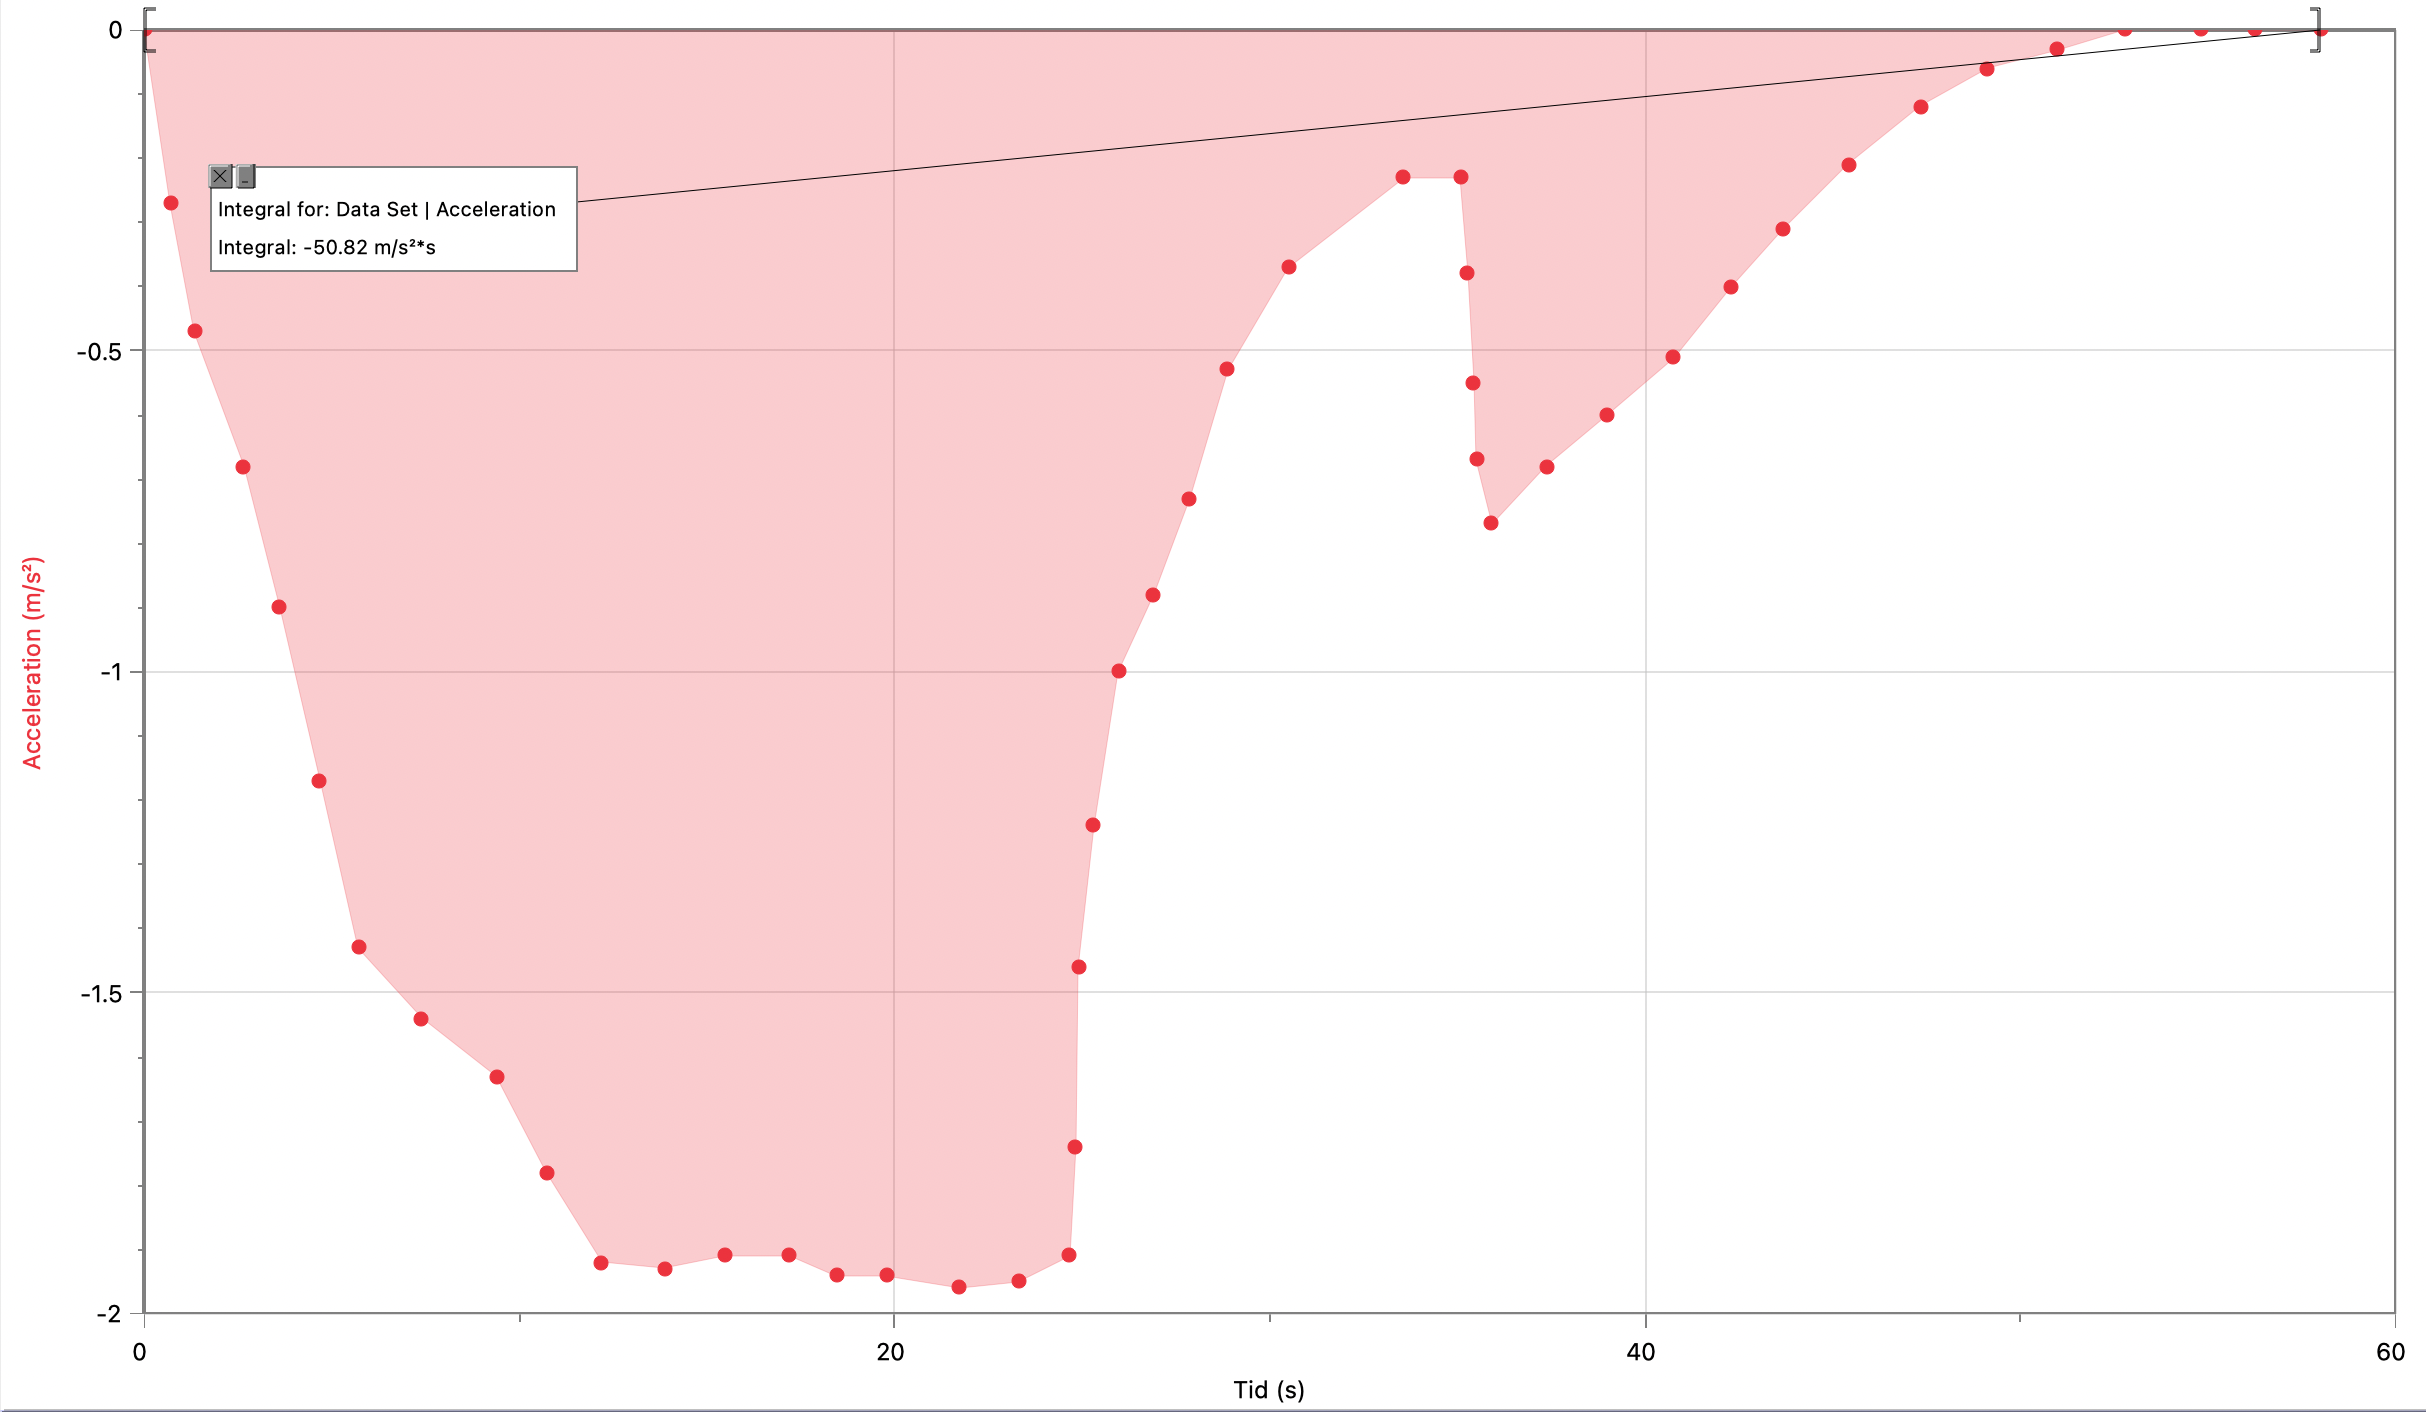
\includegraphics[width=\textwidth]{landing.png}
\end{center}
  \caption{Arealet under $(t,a)$-grafen findes i Logger Pro}
\label{fig:landing}
\end{figure}
Efter landingen har vi altså 
\[
\Delta v =-50,82 \;\unit{m/s} 
\] 
Vi kan nu udregne farten til start, hvor flyet rammer landingsbanen.
\begin{equation*}
\begin{split}
  v _{\text{start} }&=v _{\text{slut} } - \Delta v \\
  &=30 \cdot \frac{1000}{60^2} \;\unit{m/s} - \left(-50,82 \;\unit{m/s} \right) \\
  &\approx 59 \;\unit{m/s} 
\end{split}
\end{equation*}
Når flyets hjul rammer landingsbanen er dets fart altså $59 \;\unit{m/s} $.
\begin{question}{Kernekraftværk}{}
  I en fissionsreaktor bliver kølevandet bestrålet af neutroner i reaktorkernen.
  Efter indfangning af en neutron omdannes \ce{^16O} i kølevandet til \ce{^16N} og en anden partikel.
  \begin{itemize}
    \item[a.] Opskriv reaktionsskeamet for dannelsen af \ce{^16N}. Begrund, hvilken anden partikel, der dannes.
  \end{itemize}
Aktiviteten fra \ce{^16N} er ved udløbet af reaktorkernen $3,11 \cdot 10 ^{9} \;\unit{Bq/L} $. 
Når kølevandet løber ind i reaktorkernen igen, er aktiviteten fra \ce{^16N} faldet til $8,75 \cdot 10 ^{8} \;\unit{Bq/L} $.
\begin{itemize}
  \item[b.] Bestem, hvor lang tid kølevandet befinder sig udenfor reaktorkernen.
\end{itemize}
\end{question}
\sol \\
\textbf{a.}
Reaktionsskemaet for dannelsen af \ce{^16_7N} må være
\[
\ce{^16_8O + ^1_0n -> ^16_7N + ^1_1H} 
\] 
Den anden partikel, der dannes, er altså \ce{^1_1H}, hvilket er den eneste mulighed, hvis nukleontallet $A$ og ladningen $Z$ skal være bevarede.
Vi kontrollerer, at $A$, $Z$ og leptontallet $L$ er bevarede:
\begin{equation*}
\begin{split}
  A&:\; 16 + 1 = 16 +1\\
  Z&:\; 8 + 0 = 7 + 1\\
  L&:\; 0 + 0 = 0 + 0
\end{split}
\end{equation*}
Altså må \ce{^1_1H} være den anden partikel, der dannes.\\[1ex]
\textbf{b.}
Der gælder fra aktivitetens sammenhæng med tiden, at 
\begin{equation*}
\begin{split}
  A _{2}=A _{1} \cdot \left(\frac{1}{2}\right) ^{\frac{\Delta t}{T _{\frac{1}{2}}}} \iff  \Delta t = T _{\frac{1}{2}} \cdot \log_{\frac{1}{2}}\left(\frac{A_2}{A_1}\right) 
\end{split}
\end{equation*}
Ved opslag findes halveringstiden for henfaldet af \ce{^16N} til at være $T_{\frac{1}{2}}=7,1 \;\unit{s} $.\footnote{Databog, s. 200}
Vi kan nu udregne tilvæksten i tid.
Bemærk, at der her formelt set er tale om aktivitet per volumen $\frac{A}{V}$ i stedet for blot aktivitet $A$, men det ændrer ikke på resultatet, da der er tale om en intensiv størrelse. 
\begin{equation*}
\begin{split}
  \Delta t &= T _{\frac{1}{2}} \cdot \log_{\frac{1}{2}}\left(\frac{A_2}{A_1}\right) \\
  &=7,1 \;\unit{s} \cdot \log_{\frac{1}{2}}\left(\frac{8,75 \cdot 10 ^{8} \;\unit{Bq/L} }{3,11 \cdot 10 ^{9} \;\unit{Bq/L} }\right) \\
  &\approx 13,0 \;\unit{s} 
\end{split}
\end{equation*}
Altså befinder kølevandet sig $13,0 \;\unit{s} $ udenfor reaktorkernen. 
\begin{question}{Isotop af mendelevium}{}
  Isotopen $^{244}$Md blev fremstillet i en accelerator. 
  For at separere $^{244}$Md fra andre isotoper afbøjes Md$^{2+}$-ioner i et homogent elektrisk felt med størrelsen $8,47 \cdot 10^{4}$V/m.
\begin{itemize}
  \item[a.] Beregn størrelsen af kraften fra det homogene elektriske felt på en Md$^{2+}$-ion.
\end{itemize}

Isotopen $^{244}$Md er radioaktiv og henfalder ved alfa-henfald. Ved at måle på energien af de
udsendte alfapartikler bestemmer forskere henfaldets Q-værdi til $1,411\cdot $10$^{-12}$ J.
\begin{itemize}
  \item[b.] Opskriv reaktionsskemaet for det radioaktive henfald af $^{244}$Md, og benyt Q-værdien til at bestemme atommassen for isotopen $^{244}$Md.
\end{itemize}
\end{question}
\sol \\
\textbf{a.}
\ce{Md^2+}-ionerne må have en ladning på $q=2 \cdot e$. 
Vi beregner nu størrelsen af feltkraften på en \ce{Md^2+}-ion.
\begin{equation*}
\begin{split}
  F&=q \cdot E\\
  &=2 \cdot e \cdot 8,47 \cdot 10^4 \;\unit{V/m} \\
  &=2 \cdot 1,6022 \cdot 10 ^{-19}\;\unit{C} \cdot 8,47 \cdot 10^4 \;\unit{N/C} \\
  &\approx 2,71 \cdot 10 ^{-14} \;\unit{N} 
\end{split}
\end{equation*}
Størrelsen af kraften fra det homogene elektriske felt på en \ce{Md^{2+}}-ion er altså $2,71 \cdot 10 ^{-14} \;\unit{N} $.\\[1ex]
\textbf{b.}
Reaktionsskemaet for alfa-henfaldet af \ce{^244Md} må være 
\[
\ce{^244_101Md -> ^240_99Es + ^4_2He} 
\] 
Vi kontrollerer, at nukleontallet $A$, ladningen $Z$ og leptontallet $L$ er bevarede:
\begin{equation*}
\begin{split}
  A&: \; 244=240+4\\
  Z&: \; 101=99+2\\
  L&: \; 0=0+0
\end{split}
\end{equation*}
Vi vil nu finde et udtryk for for atommassen af \ce{^244Md}.
\begin{equation*}
\begin{split}
  Q=-\Delta m \cdot c^2 &\iff Q=-\left(\left(m \left(\ce{^240_99Es}\right) -99 \cdot m_e\right) + \left( m(\ce{^4_2He} )-2 \cdot m_e\right)-\left(m \left(\ce{^244_101Md}\right)  -101 \cdot m_e\right) \right) \cdot c^2\\
  &\iff -m (\ce{^240_99Es}) - m(\ce{^4_2He} )+m (\ce{^244_101Md})=\frac{Q}{c^2}\\
  &\iff m (\ce{^244_101Md})=\frac{Q}{c^2}+m (\ce{^240_99Es}) + m(\ce{^4_2He} )
\end{split}
\end{equation*}
Vi beregner nu atommassen af \ce{^244Md}.
\begin{equation*}
\begin{split}
  m (\ce{^244_101Md})&=\frac{Q}{c^2}+m (\ce{^240_99Es}) + m(\ce{^4_2He} )\\
  &=\frac{1,411 \cdot 10 ^{-12} \;\unit{J} }{1,4924 \cdot 10 ^{-10} \;\unit{J/u} } + 240,06892 \;\unit{u} + 4,002603254 \;\unit{u} \\
  &\approx 244,1 \;\unit{u} 
\end{split}
\end{equation*}
Atommassen for isotopen \ce{^244Md} er altså $244,1 \;\unit{u} $.
\begin{question}{Bevægelse i homogent elektrisk felt}{}
  To parallelle metalplader anbringes i vakuum, så afstanden mellem dem er er 1,70 cm, og spændingsfaldet mellem dem er 34 V.
  \begin{itemize}
    \item[a.] Beregn størrelsen af det elektriske felt mellem pladerne.
  \end{itemize}
På figuren nedenfor ses til venstre en elektronkanon, som accelererer elektronerne fra hvile ved at lade dem gennemløbe et spændingsfald på 220 V.
\begin{itemize}
  \item[b.] Hvilken fart opnår elektronerne ved denne acceleration?
\end{itemize}
Elektronerne bliver afbøjet af det elektriske felt. (Vi skal undgå at elektronerne rammer den positive ladet plade).
\begin{itemize}
  \item[c.] Bestem hvor lange de to metalplader må være, hvis elektronerne skal ”slippe gennem”.
\end{itemize}
\end{question}
\sol \\
\textbf{a.}
Vi beregner størrelsen af det elektriske felt mellem de to plader.
\begin{equation*}
\begin{split}
  E&=\frac{U}{d}\\
  &=\frac{34 \;\unit{V} }{1,70 \cdot 10 ^{-2} \;\unit{m} }\\
  &=2,0 \cdot 10 ^{3} \;\unit{V/m} 
\end{split}
\end{equation*}
Størrelsen af den elektriske feltstyrke mellem pladerne er altså $2,0 \cdot 10^3 \;\unit{V/m} $.\\[1ex]
\textbf{b.}
Afstanden mellem katoden og anoden på kanonen betegner vi $s$ og spændingsforskellen betegner vi $U _{\text{kanon} }$.
Siden feltkraften fra kanonen er den eneste kraft, der påvirker en elektronen mens den er i kanonen, så har vi 
\begin{equation*}
\begin{split}
  A _{\text{res} }&=A _{\text{kanon} }\\
  &=F _{\text{kanon} } \cdot s \\
  &=E _{\text{kanon} } \cdot e \cdot s\\
  &=\frac{U _{\text{kanon} }}{s} \cdot s \cdot e \\
  &=U _{\text{kanon} } \cdot e
\end{split}
\end{equation*}
hvor $e$ er elementarladningen. 
Da $A _{\text{res} }=\Delta E _{\text{kin} }$, og elektronerne accelereres fra hvile, så har vi 
\begin{equation*}
\begin{split}
  U _{\text{kanon} } \cdot e= \frac{1}{2} \cdot m_e \cdot v^2 \iff v=\sqrt{\frac{2 \cdot e \cdot U _{\text{kanon} }}{m_e}} 
\end{split}
\end{equation*}
Vi udregner nu den fart, som elektronerne opnår.
\begin{equation*}
\begin{split}
  v&=\sqrt{\frac{2 \cdot e \cdot U _{\text{kanon} }}{m_e}} \\
  &=\sqrt{\frac{2 \cdot 1,6022 \cdot 10 ^{-19} \;\unit{C} \cdot 220 \;\unit{V}}{9,1094 \cdot 10 ^{-31} \;\unit{kg} }} \\
  &\approx 8,80 \cdot 10^6 \;\unit{m/s} 
\end{split}
\end{equation*}
Ved accelerationen opnår elektronerne altså farten $8,80 \cdot 10^6 \;\unit{m/s} $.\\[1ex]
\textbf{c.}
Vi finder først et udtryk for tiden $t$ det tager for elektronen at være på niveau med den positive plade.
Vi ser bort fra tyngdekraften, og den eneste kraft, der påvirker elektronen er da feltkraften $F$, som påvirker elektronen vertikalt i retning mod den positive plade.
Fra Newtons anden lov har vi så
\begin{equation*}
\begin{split}
  a=\frac{F}{m_e}=\frac{e \cdot E}{m_e}
\end{split}
\end{equation*}
Vi ser, at accelerationen er konstant.
Siden elektronens vertikale fart til start er $0$, så har vi, at når elektronen er på samme nivau ($y$-værdi) som pladen, så gælder 
\begin{equation*}
\begin{split}
  \frac{1}{2} d =\frac{1}{2} \cdot \frac{e \cdot E}{m_e} \cdot t^2 \iff t=\sqrt{\frac{d \cdot m_e}{e \cdot E}} 
\end{split}
\end{equation*}
Da elektronen ikke accelereres i vandret retning, er der tale om en jævn bevægelse i vandret retning.
Vi kan nu beregne, hvor langt elektronen når, inden den når samme højde som den positive plade.
\begin{equation*}
\begin{split}
  x&=v_x \cdot t \\
  &=v_x \cdot \sqrt{\frac{d \cdot m_e}{e \cdot E}} \\
  &=8,7971 \;\unit{m/s} \cdot \sqrt{\frac{1,70 \cdot 10 ^{-2} \;\unit{m} \cdot 9,1094 \cdot 10 ^{-31} \;\unit{kg} }{1,6022 \cdot 10 ^{-19}\;\unit{C} \cdot 2,0 \cdot 10^3 \;\unit{V/m} }} \\
  &\approx 0,061 \;\unit{m} \\
  &=6,1 \;\unit{cm} 
\end{split}
\end{equation*}
Altså må metalpladerne højst være $6,1 \;\unit{cm} $ lange, hvis elektronerne skal slippe igennem. 
\begin{question}{Rheostat}{}
  En rheostat, der er indstillet til resistansen 430 $\Omega$, indsættes i et elektrisk kredsløb
Spændingsfaldet over rheostaten er 90 V.
\begin{itemize}
  \item[a.] Beregn strømstyrken gennem rheostaten.
\end{itemize}
Rheostaten anvendes i en lysdæmper til en glødepære, som vist i diagrammet.
Grafen viser effekten $P$, hvormed glødepæren omsætter energi, som funktion af strømstyrken $I$
gennem pæren.
Lysstyrken dæmpes, så pærens effekt er 35 W.
\begin{itemize}
  \item[b.] Bestem resistansen af rheostaten, når pærens effekt er 35 W.
\end{itemize}
\end{question}
\sol \\
\textbf{a.}
Da der er tale om en resistor, så gælder Ohms lov.
\begin{equation*}
\begin{split}
  U=R \cdot I \iff I=\frac{U}{R}
\end{split}
\end{equation*}
Vi beregner nu strømstyrken gennem rheostaten.
\begin{equation*}
\begin{split}
  I&=\frac{U}{R}\\
  &=\frac{90 \;\unit{V} }{430 \;\unit{\ohm} }\\
  &\approx 0,21 \;\unit{A} 
\end{split}
\end{equation*}
Strømstyrken gennem rheostaten er altså $0,21 \;\unit{A} $.\\[1ex]
\textbf{b.}
Vi aflæser på $(I,P)$-grafen (se \cref{fig:IP}), at når pærens effekt er $35 \;\unit{W} $, så er strømstyrken gennem den $0,22 \;\unit{A} $.
Vi kan nu finde et udtryk for spændingsfaldet over pæren.
\begin{equation*}
\begin{split}
  U _{\text{pære} }&=\frac{P _{\text{pære} }}{I}
\end{split}
\end{equation*}
Siden pæren og rheostaten er serieforbundne, så er strømstyrken $I$ konstant og det samlede spændingsfald må være $U=U _{\text{rheostat} } + U _{\text{pære} }$.
Rheostatens resistans må da være
\begin{equation*}
\begin{split}
  R _{\text{rheostat} }&=\frac{U _{\text{rheostat} }}{I}\\
  &=\frac{U-U _{\text{pære} }}{I}\\
  &=\frac{U-\frac{P _{\text{pære} }}{I}}{I}\\
  &=\frac{230 \;\unit{V} - \frac{35 \;\unit{W} }{0,22 \;\unit{A} }}{0,22 \;\unit{A} }\\
  &\approx 3,2 \cdot 10^2 \;\unit{\ohm} 
\end{split}
\end{equation*}
Resistansen af rheostaten er altså $3,2 \cdot 10^2 \;\unit{\ohm}$, når pærens effekt er $35 \;\unit{W} $.
\begin{figure}[H]
\begin{center}
  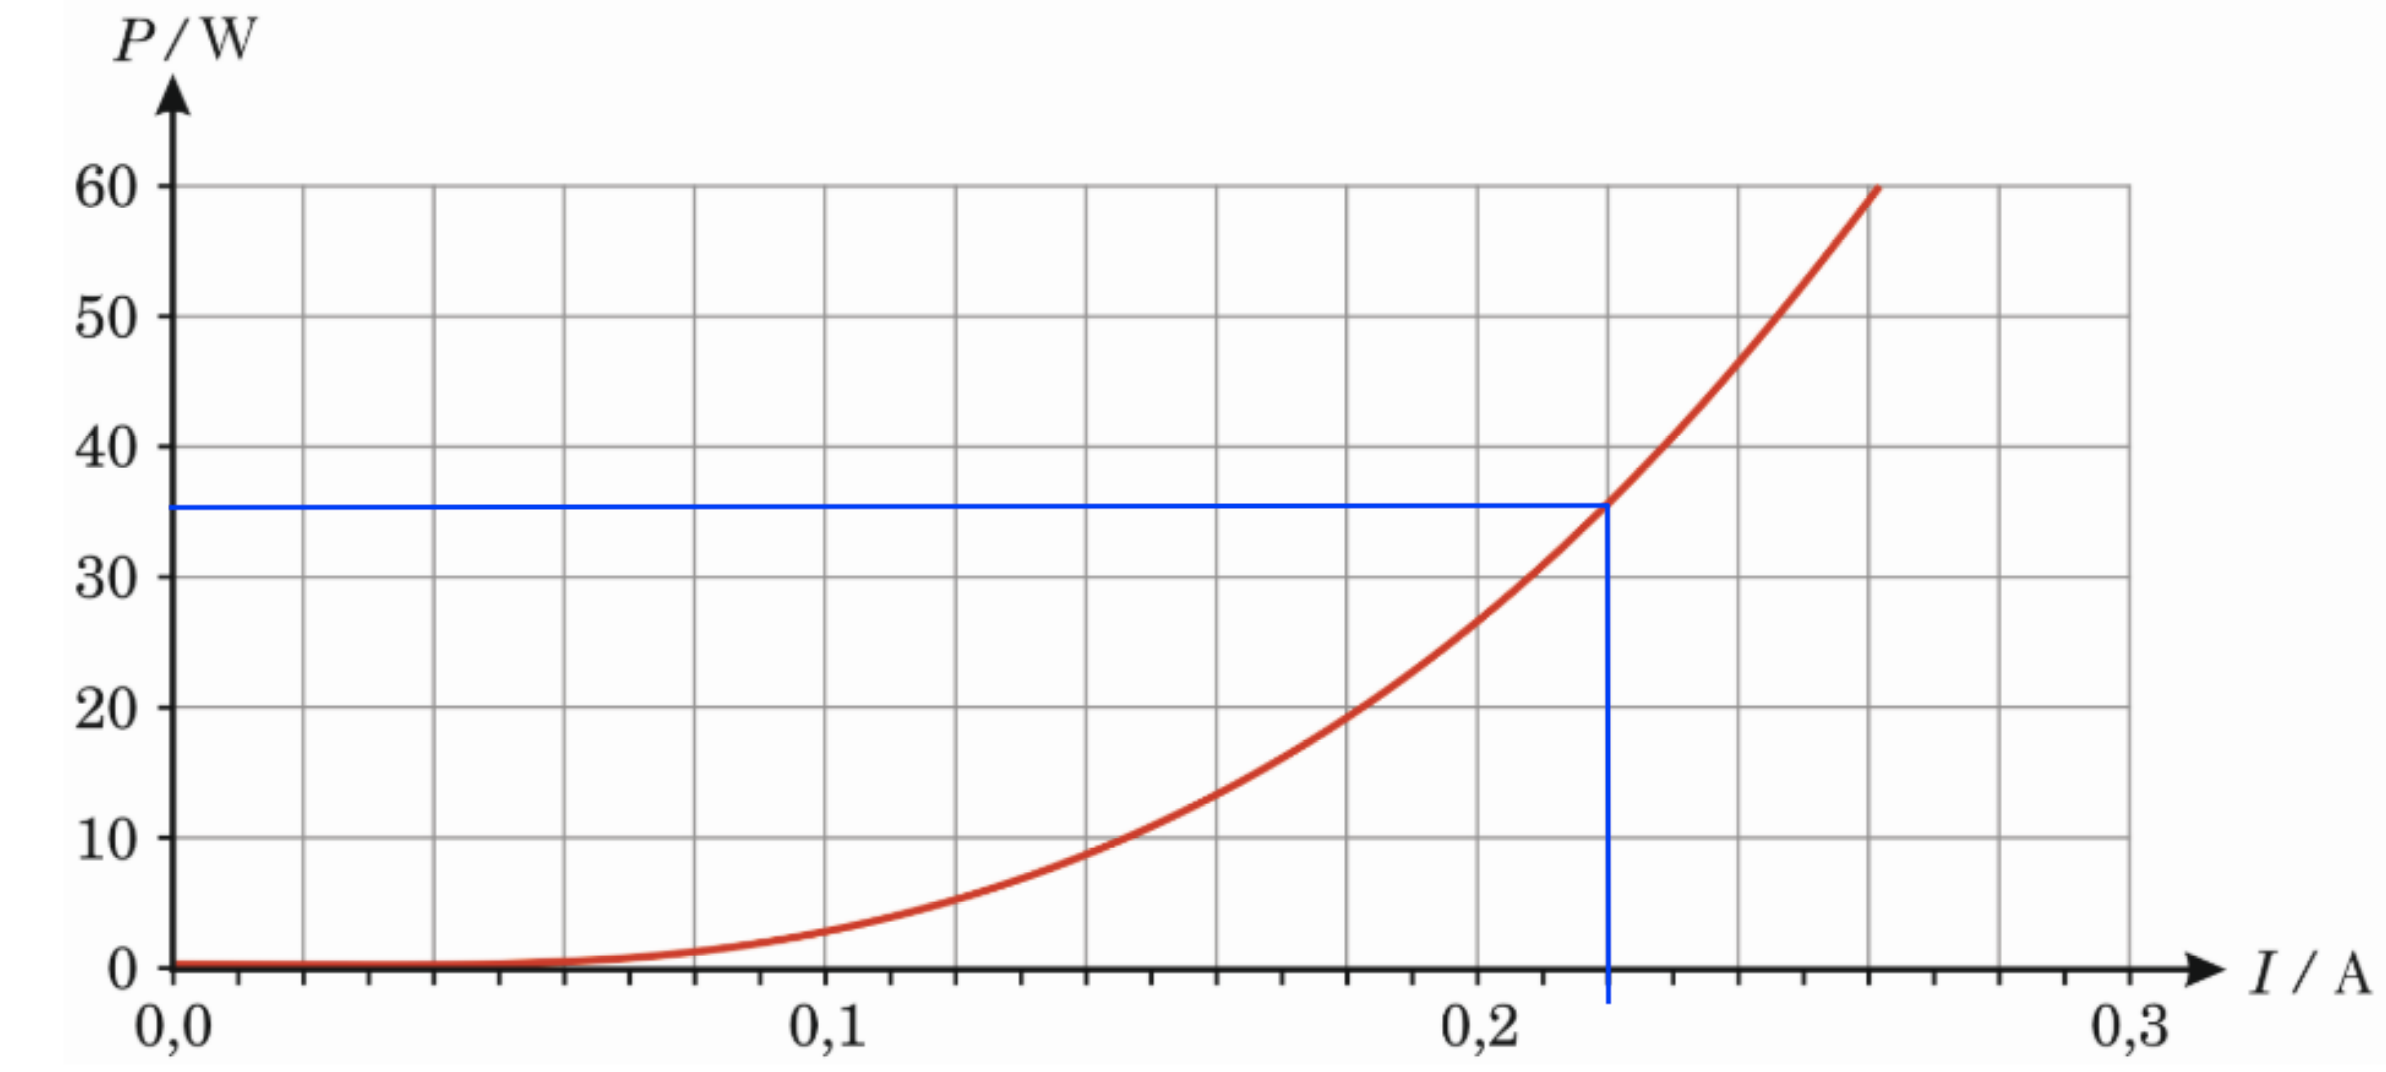
\includegraphics[width=\textwidth]{IP.png}
\end{center}
  \caption{Aflæsning på (I,P)-grafen for pæren}
\label{fig:IP}
\end{figure}

\end{document}
